

\ifx \definition \undefined
	\newtheorem{definition}{Definition}
\fi
\ifx \conjecture \undefined
	\newtheorem{conjecture}{Conjecture}
\fi

\chapter{Diagnosis-oriented Modeling and Verification Framework}
\label{chap:framework}

This first part of the chapter presents a modeling approach for design of
manufacturing systems which exploits idea of decomposition of a system into modules, and presents them
in a form of UML blocks. It is shown then, how the modules are
represented internally by automata, and how the failures can be modeled. The
second part of this chapter gives a necessary introduction into a formal
notation for discrete event systems in terms of languages and automata,
and describes different types of diagnosability.

\section{Modeling Framework}

\subsection{Introduction}

The fundamental principle ``divide and concur'' underlies many techniques and
approaches either used solely at the level of individual engineers and
programmers or developed at the level of international standard committees and
organisations. For instances, one can recall object-oriented concepts in
traditional programming principles \cite{farrell_object-oriented_2013}, and
standards of International Electrotechnical Commission (IEC), particularly the
legacy IEC 61131-3 \cite{otto_iec_2009} which defines programming languages for
programmable logic controllers (PLC), and the modern IEC 61499
\cite{vyatkin_iec_2009} which represents a component solution for distributed
industrial automation systems aiming at portability, reusability,
interoperability and reconfiguration of distributed applications.

Many Integrated Development Environments (IDE) used in industrial world satisfy
all the requirements and standards in order to facilitate the process of
development, enrollment and maintenance of a complex system. They exploit
object-oriented concepts as classes with their instances, inheritance and
encapsulation (for instance, as in  \cite{serna_design_2010},
\cite{steinegger_design_2013} and \cite{zoitl_guidelines_2013}). However, these
concepts were not initially created bearing in mind the purpose of formal
verification. As a consequence, the tools widely used in industry nowadays do
not generally support approaches for DES raising in the scientific world. As a
response for the growing demand for intersection of classical development
process with formal techniques many researches attempt to create instrumental
and theoretical bridges. The most promising results seem to be reached in
formalizing Unified Modeling Language (UML), Statecharts, and general purpose
programming languages as C.

\begin{figure}[t]
	\centering
	\includegraphics{uml_state_machine.png}
	\begin{tikzpicture}[->,>=stealth, node distance=4cm, auto, shorten >=1pt,
	semithick, initial text=,	
		every node/.style={scale=0.8},
		every state/.style={minimum size=2.2cm},
	    accepting/.style={double distance=1.5pt, outer sep=0.75pt+\pgflinewidth}
	    ]
% \draw[help lines] (0,0) grid (6,2);
	\node[state]         (1) [] 	  {toasting};
	\node[state]         (3) [below of=1]       {door~open};
	\node[state]         (2) [below of=3]       {baking};
	\node[] (0') [left of=3] {}; %dummy
	\node[initial,state] (0) [left of=0']{initial};
	\node[above = 1em of 1] {}; %adds some space above
	\path
	(0)	edge [bend left, align=left]  node [above left]
		{ do\_toasting / \\ heater\_on \\  arm\_time\_event	}
	(1) 
	(0)	edge [bend right, align=left]  node [below left] 
		{ do\_baking / \\ heater\_on \\ set\_temperature }
	(2)
	(1)	edge [bend left, align=left]  node [right]
		{ door\_open / \\ heater\_off \\ disarm\_time\_event \\ lamp\_on }
	(3) 
	(3)	edge [bend left, align=left]  node [left]
		{ door\_close / \\ heater\_on \\ arm\_time\_event \\ lamp\_off }
	(1) 
	(2)	edge [bend right, align=left]  node [right]
		{ door\_open / \\ heater\_off \\ set\_temperature\_0 \\ lamp\_on }
	(3) 
	(3)	edge [bend right, align=left]  node [left]
		{ door\_close / \\ heater\_on \\ set\_temperature \\ lamp\_off }
	(2) 
	;
	\end{tikzpicture}

	\caption{Example of an UML Statechart diagram (at top) and its representation
	by the Mealy automaton}
	\label{fig:example_of_UML_with_Mealy}
\end{figure}

In \cite{mcumber_general_2001} the authors introduce a framework which allows to
convert an UML model into the formal languages described in the form of
specification. The framework can be applied only for a subset of UML diagrams.
The resulting formal specification can be used for model checking and
simulation, using existing tools aimed for this purpose. Figure
\ref{fig:example_of_UML_with_Mealy} depicts the instance of an UML diagram and
its representation by a Mealy automaton which, in its turn, can be transformed
into a classical automaton. In \cite{bonfe_design_2003} the authors develop a
framework to transform UML diagrams and Statecharts into Computation Tree Logic
(CTL) which is the used in a model checking tool.
Other works to mention are \cite{dong_model_2001}, where UML diagrams are mapped
to automata, \cite{frey_re-engineering_2004} where the authors concentrate on
converting PLC languages to UML and then to automata. Even a such known widely
spread tool as Matlab \cite{matlab}, used by both practitioners and
theoreticians, also has to be tweaked in order to get its modeling ability
closer to a formal representation. Examples of such attempts are
\cite{ray_automated_2007} and \cite{li_stateflow_2011}. An instance of model
checking tool, which is exploited by many of the approaches mentioned above, the
most notable one is NuSMV \cite{nusmv} which automatically verifies properties
of finite-state systems, expressed in CTL, Linear Temporal Logic (LTL) or
Property Specification Language (PSL).

Quick analysis of the aforementioned attempts to bridge the most widely
used object-oriented IDEs and their underlining modeling technologies shows that
they solve the problem of using formal methods by system's developers
only partially. The reason is, as it was said before, that those concepts
and tools had been developed before formal methods became useful in practice,
and they simply can not be merged with modern formal approaches. The problem
lays, firstly, in the ambiguity of legacy methods, their freedom of
interpretation. It appears when, for instance, one tries to convert an UML
diagram to automata. Second, the problem comes from the fact, that producers of
development tools have created a wide range of derivatives of one standard,
which, at one hand, satisfied requirements of the market and, on the other hand,
made these implementations incompatible to each other. Now, when formal
approaches both, have reached enough theoretical level, and have growing demand
due to the high complexity of currently appearing systems, there is a need for
new approaches and tools that exploit formal methods as an underlying concept.

One of the approaches which uses the object-oriented principles, and focuses on
formal verification is presented in \cite{sartini_architectures_2010}. The
approach introduces a modeling entity called \emph{Generalized Device} and shows
how it can be used for formal verification in the DES framework. The approach is a
refined architecture of a concept of \emph{Generalized Actuator} for industrial
automated systems \cite{faldella_hierarchical_2008}. The next section gives a
brief introduction into both the concept and the refined approach.


\subsection{Generalized Actuator and Generalized Device}

\subsubsection{Generalized Actuator}

The GA approach aims to reduce complexity of the modeling process using
standardized object-oriented concepts of engineering.
An idea of GA is to identificate essential patterns in automated manufacturing
systems, and design control software entities suitable for formal methods of DES
theory. The GA approach gives a modeling framework and defines a design
procedure with following characteristics:
\begin{itemize}
  \item Encapsulation of ``actuation mechanism'';
  \item Hierarchical representation of a plant;
  \item Separation of control policies from actuation mechanisms in each GA;
  \item Support of visualization of plant's hardware;
  \item Interoperability and reusability of GAs.
\end{itemize}

\begin{figure}[!t]
	\centering
	\includegraphics[width=30em]{ga_blocks.png}
	\includegraphics[width=30em]{ga_automaton.png}
	\caption{GA with two types of interfaces (top) and its underlining
	formal representation by the automaton (bottom)}
	\label{fig:ga_blocks}
\end{figure}

The GA implements a concept of abstraction. It implies that all the actions of a
complex process, from the high-level point of view, can be decomposed into sets
of two kinds: \emph{Do-Done} actions and \emph{Start-Stop} actions.

The Do-Done GA reflects a process which starts by an external (with respect to
this process) ``Do'' command, and continues until an internal (with respect to
this process) decision to terminate is taken. The duration can be finite or
infinite. After its termination the process issues ``Done'' event. The 
instance of a process which can be abstracted by this type of GA is the opening
of a valve: the command ``Do'' is issued to open the valve; when it opens, the
event ``Done'' occurs.

The Start-Stop GA is an abstraction of a process which starts by an external
``Start'' event, and continues until an external ``Stop" event occurs .
Again, the duration can be finite or infinite. The instance of a such process is
a temperature regulation with a heater: the ``Start'' event switches on the
heater; when temperature reaches a required level the ``Stop'' event switches it off.

The above described two types of GA can be implemented as Functional Blocks
(FB) in terms of IEC 61131-3 standard, as depicted in Figure
\ref{fig:ga_blocks}
\footnote{The image is borrowed from \cite{faldella_hierarchical_2008}}. 
Besides the essential inputs and outputs necessary to perform the above described types of actions, the blocks have other inputs and
outputs related to the low level of processes, and to some additional
information related to the high level. 

Internally, each type of GA is represented by the automaton, as depicted on the
figure. Each state of the automaton can abstract a set of states of other
automata, i.e. GAs contain a hierarchical structure of automata.

A design procedure, according to the framework of GA can be described by the
following steps:
\begin{itemize}
  \item Identification of distinguished processes and their basic actions;
  \item Classification of actions into Do-Done and Start-Stop actions;
  \item Definition of GAs for two kinds of actions;
  \item Assigning low level information and additional information to each GA;
  \item Design of internal hierarchical structure and logic of automata for
  each GA.
\end{itemize}

The last two steps in the above described design procedure encapsulate a logic
specific for a given process. Potentially, the complexity of internal
implementations of GAs is not limited. Thus, the functional blocks
corresponding to the GAs can became very specific, such that it would be
possible to reuse them only at the same plant, or for a technologically similar
processes. A designer of a GA must be aware of this problem, and maintain
simplicity of the internal implementation. Instead of increasing the complexity
of internal structure of a GA, one can create other GAs. However, this
process relies solely on decision of a particular designer for a system.

The design problem, described above, can be reformulated as that a GA abstracts
a process at its high level, but does not abstract it at its low level. The
architectural approach of Generalized Device (GD) is aimed to solve this
problem.

\subsubsection{Generalized Device}

The idea of a Generalized Device is based of the observation that the most
of different low level field devices can be viewed as only two kind of abstract
devices: either single acting device or double acting device. Each kind
of devices has an actuator and also may have sensors.

A single acting device has only one command (input) to perform a ``forward'' or
``on'' action. The ``backward'' or ``off'' action is performed by the device
itself, implicitly ore explicitly. Examples of single acting devices are:
a cylinder with a return spring, a contactor itself or together with any
controlled equipment (electric motor, heater, lighting, etc).

A double action device has one command to activate the device and another
command to deactivate it. Simultaneous commands on inputs of the device are
usually prohibited or have now effect on a state of the device. The instances of
double action devices are: a double acting cylinder, an auxiliary relay or any
start-stop device which may itself be a composition of two single acting
devices.

The common feature of the both, single and double acting devices is that they
have two clearly distinguished states. In order to detect what the current state
of a device stays in, it is usually equipped with one or two sensors. In case of
two sensors each of them gives the feedback for the corresponding state. In case
of one sensor one level of its signal corresponds to the first state of the
device, another level - to the second one. A state of the device in the case
when it has no sensors is implied according to a previous command. Concluding,
a classification of the devices in this approach is the following:

\begin{itemize}
  \item Single acting device
	\begin{itemize}
	  \item with no feedback
	  \item with single feedback
	  \item with double feedback
	\end{itemize} 
  \item Double acting device
	\begin{itemize}
	  \item with no feedback
	  \item with single feedback
	  \item with double feedback
	\end{itemize} 
\end{itemize} 


\begin{figure}[t]
	\centering
% 	\includegraphics[width=30em]{dadf.png}
	\includegraphics[width=30em]{dadf.pdf}
	\caption{Device with Double Actuation and Double Feedback (DADF) and its
	connection to a physical device (valve)}
	\label{fig:dadf}
\end{figure}
 
As an instance, the Figure \ref{fig:dadf} depicts the device with double
activation and double feedback. It abstracts a physical device, the valve
in this example, for a higher level GA.

\begin{figure}[t]
	\centering
	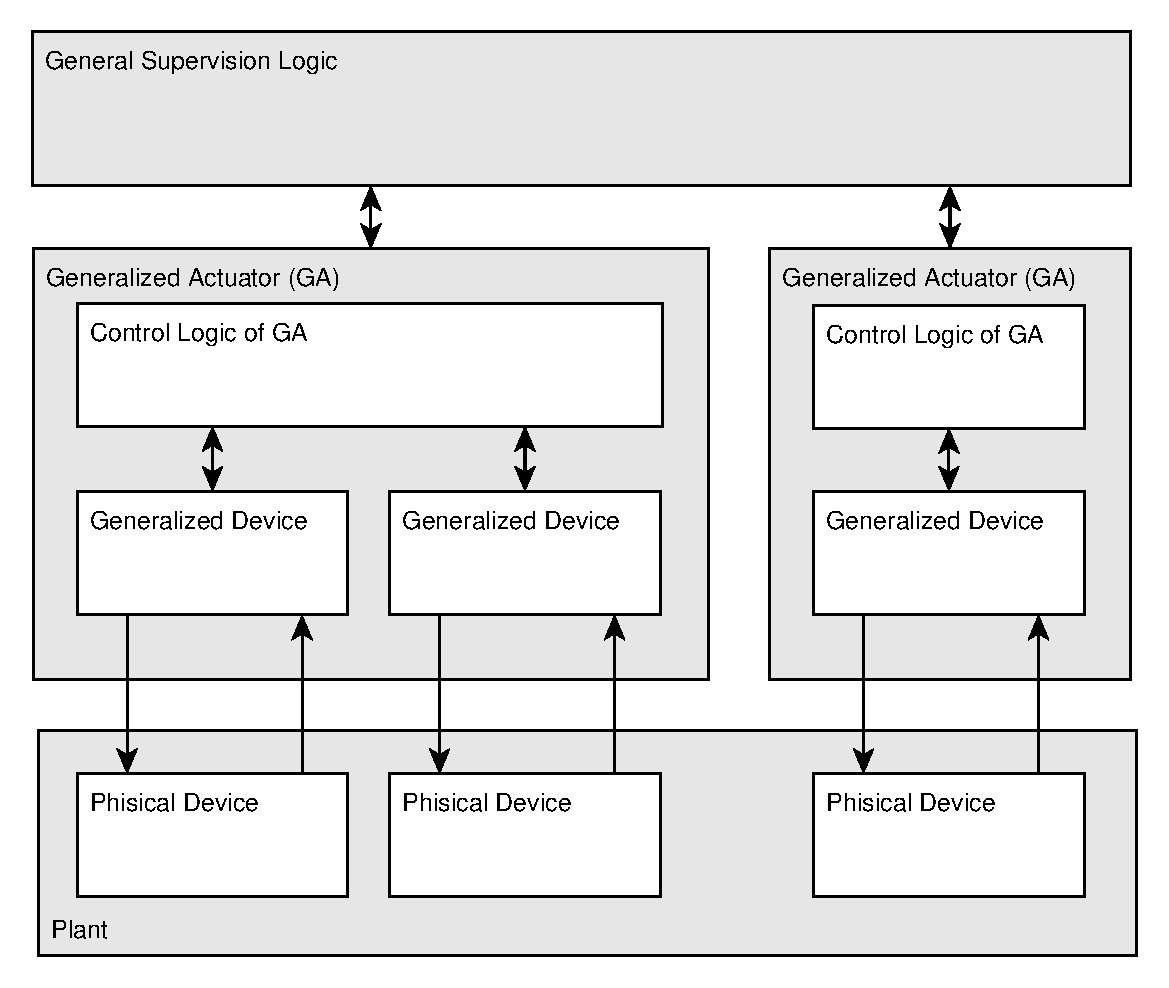
\includegraphics[width=30em]{levels_ga_gd.pdf}
	\caption{Hierarchical relation of system's components: high level logic of
	plant, GAs, GDs and physical devices}
	\label{fig:levels_ga_gd}
\end{figure}

The approach of generalized actuators and devices allows to construct complex
automated systems using simple predefined models, as it is shown at the Figure
\ref{fig:levels_ga_gd}.
  
Due to representation of the system's models by automata, various DES techniques
can be applied in order to define and solve control and diagnosis problems for
entire system. To preserve the level of abstraction, however,
additional information necessary for a required problem has to be encapsulated
into modules. Particularly, possible failure behaviour should be incorporated
into modules for the diagnosability problem.

The next section proceeds with a description of how the approach of generalized
device is used for modeling and analyses of faults.


\subsubsection{Generalized Device and Failures Diagnosis}

This section briefly describes an approach for building structured formal
models, presented in \cite{sartini_methodology_2010}. The methodology extends
the approach of generalized device to facilitate diagnosis verification
and monitoring problems. The authors present each GD as a composition of
automata, where automata reflect control logic and a model of physical device,
decomposed into sensors, actuators, components and their constrains. For the
sake of simplicity, the approach is presented further with a small illustrative
example. The example shows the idea of decomposition with two components of a
hypothetical device (think of a valve from the system given in Chapter
\ref{chap:problem_description}), their constrains and how failures are modeled.

\begin{figure}[t]
	\centering
	\includegraphics[scale=0.8]{do.pdf}
	\caption{Automaton representing digital output}
	\label{fig:do}
\end{figure}

The Figure \ref{fig:do} depicts a model of digital output (a
model of digital input would be equal). The automaton has two states,
reflecting the low and high levels of signal. The event labels of the automaton
are corresponding to digital signal states as shown in the table
\ref{tbl:do_events}. The states of a signal are treated as events because
they are seen as readings (two values) of a variable (either it is output or
input) in a program in PLC, while the cyclical program execution.

\begin{table}[t]
\caption{Correspondence of automata event labels to digital output signals}
\centering
	\begin{tabular}{l l}
	\\	
	Label & Digital output signal state\\
	\hline
	do\_lo & Digital output signal is low\\
	do\_hi & Digital output signal is high\\
	\end{tabular}
	\label{tbl:do_events}
\end{table}

\begin{figure}[t]
	\centering
	\includegraphics[scale=0.7]{./figures/relay.pdf}
	\includegraphics[scale=0.7]{do2relay.pdf} 
	\includegraphics[scale=0.7]{do+relay.pdf} 
	\caption{Automata models of Relay (top left, constrains (top right), and 
	result of composition (bottom)}
	\label{fig:do+relay}
\end{figure}

In major of cases, a digital output is linked to an actuator, there is an
intermediate signal amplifier, e.g. an electromagnetic relay. It acts also as an
galvanic isolation of the PLC and the field device. 

In this example, the behaviour of the relay is related to the behaviour of
digital output, i.e. it is constrained by the digital output. A model of the
relay, a model of constrain and the resulting composition of all the
aforementioned components is depicted in the Figure \ref{fig:do+relay}.

\begin{figure}[t]
	\centering
	\includegraphics[scale=0.7]{relay_f0.pdf}
	\caption{Failure model of the relay (example of the broken coil) }
	\label{fig:relay_f0}
\end{figure}s

For illustration of a failure lets pick one of the possible relays failures,
e.g. broken coil. The corresponding model of the relay with this failure is
depicted in the Figure \ref{fig:relay_f0} (event $f0$ states for the failure
event). Similar to the this failure, a ``stuck on'' relay's failure can be
modeled.

As the the approach of GD assumes, almost any field device can be decomposed
into simple components, as ones described in the above example. The failure
models for such components can be easily determined. More complex components can
be then composed by using the simple models and constrain automata. Thus, a
set of predefined models can be exploited for building a library of GD. Since
all the models include failure behaviour, formal diagnosability analysis
techniques can be applied.

In the Chapter \ref{chap:theory} a part of the work is devoted to an extension
of the above failure modeling approach such that a failure behaviour can be
modeled without failure events, by state marking. It will be shown how a failure
behaviour can be separated from a non-failure one automatically, for further
diagnosability analysis.
 

\section{Discrete Event Systems Framework for Diagnosability Verification}

\subsection{Introduction}

Discrete Event Systems (DES) are systems, the dynamic of which is characterized
by asynchronous occurrence of \emph{events}. An event is a fundamental concept
which can be viewed and described as ``something happened'', either in systems
designed by humans or in nature. Events have no property of continuation, they
are instant, and can be observed only at discrete points in time. The second
fundamental concept, characterizing a DES, is a state. A state is viewed as a
result of \emph{temporally ordered} discrete events, occurred starting from a
moment when the system was at its \emph{initial state}. The initial state of a
DES characterizes the system before occurrence of any event. In reality, this
characteristic may be seen as an assumption or ``agreement'' for the given
system. Being at a certain state, when an event occurs, the system makes a
\emph{transition} to another state.

The examples of events are: switching a light on, pressing a button, a 
moment of rising a temperature above a certain level. The corresponding states
are: the light is on, the button is down, the temperature is high.

Historically, all the system's events are thought as of an \emph{alphabet}.
Temporally ordered, they form \emph{words} which, consequently, form a
\emph{language}. At this level of abstraction DES are studied by the
\emph{language theory} \cite{aho_theory_1968}.

Formal language theory is closely related to \emph{Automata theory}
\cite{hopcroft_introduction_2007}. Automata are used as one of the modeling
formalisms for DES. A single automaton can be represented as a directed graph,
and it is, probably, the simplest way a complex system's behaviour can be graphically
and formally described and conceived by humans.

The next section gives the preliminaries from theories of languages and
automata, used in this document.


\subsection{Notation}

The notation used in this document is the one in
\cite{cassandras_introduction_2010}. For the benefit of the reader we place here
the most essential notation necessary for understanding of the further material.

Let $\Sigma$ be a finite set of events. A sequence of events is a string.
$\Sigma^*$ denotes a set of all finite strings over $\Sigma$.
$L\subseteq\Sigma^*$ is a language over $\Sigma$. Given strings $s$ and $t$,
$st$ is their concatenation. Given strings $s$ and $w$, $w$ is a prefix of $s$
if it exists $t$ such that $wt = s$. Prefix closure of $L$, denoted by
$\overline{L}$ is a set of all prefixes of all the strings in $L$.
If $\overline{L} = L$ then $L$ is prefix-closed. The post language of $L$ after
a string $s$ is denoted as $L/s$, i.e. $L/s := \{t\mid st \in L\}$. We
write $\sigma \in s$ if the event $\sigma \in \Sigma$ appears in the string $s
\in \Sigma^*$. If $\{s\}$ is a singleton, we write $s$ for operations on
languages.

An automaton $G$ is a tuple $$G := \left< X,\Sigma,\delta,x_0, X_m \right>,$$
where $X$ is a set of states, $x_0 \in X$ is an initial state, $X_m \subseteq X$
is the set of marked states, and $\delta: X \times \Sigma \rightarrow X$ is the
transition function.
We say a language $L := \mathcal{L}(G)$ is generated or recognized by the
automaton $G$. In this paper we assume that for each language there is always a
corresponding automaton, and vice versa. The marked language $L_m \subseteq L$
is intended to make a part of the automaton's behaviour distinguishable in a
certain context.

Some events of DES can not be observed. To reflect that the set of events
$\Sigma$ is partitioned into disjointed sets of observable events $\Sigma_o$ and
not observable events $\Sigma_{ou}$, i.e. $\Sigma = \Sigma_o~\dot{\cup}~
\Sigma_{ou}$.
$M: \Sigma^* \rightarrow \Sigma_o^*$ denotes natural projection that
erases unobservable events.
% ; $\epsilon$ means the empty string. 
The corresponding inverse projection is $M^{-1}: \Sigma_o^* \rightarrow
2^{\Sigma^*}$.

Let $I := \{1,2,\ldots,n\} \subset  \mathbb{N}$ be an index set. A system is
defined by a set of automata $\{G_{i \in I}\}$ and a corresponding set of
languages $\{L_{i \in I}\}$. We use the term \emph{local} in context of the
automata and languages from these sets. The \emph{global} language of the system
is defined by the parallel composition \cite{cassandras_introduction_2010} of
its local languages:
$L := \parallel_{i \in I} L_i$.
The natural projection for the local languages is defined as 
$P_i := \Sigma^* \rightarrow \Sigma_i^*$. We extend it to the system's languages
as follows: $P_i(L) := \{s\mid s\in L_{i}\}$, and 
$P_i^{-1}(L_{i}) := \{s \mid s \in L, P_i(s) \in L_i\}, ~i \in I$.
We also define natural projection over observable events for the index set: 
$M_i :\Sigma_i^* \rightarrow \Sigma_{i,o}^*$, natural projection over common
events:
$P_{i,c} : \Sigma_i^* \rightarrow (\Sigma_i \cap \bigcup_{j\neq
i}^I\Sigma_j)^*$, and natural projection over observable and common events:
$P_{i,co} : (\Sigma_i \cup \Sigma_o)^* \rightarrow (\Sigma_{o} \cup (\Sigma_i
\cap \bigcup_{j\neq i}^I\Sigma_j))^*$. All the above projections, as well as
the corresponding inverse projections, are defined also for languages in the
usual manner.


\subsection{Abstraction by decomposition}

For model checking and verification of DES the state explosion problem is one of
the main limitations for their application in industry. The most important
technique to deal with the state explosion problem is abstraction. The basic
idea of abstraction is that some parts of a given system \emph{do not have
effect} on particular properties, and hence, these parts can be
\emph{eliminated} from the system's design.

One of the most effective abstraction techniques, compositional reasoning
\cite{berezin_compositional_1998}, deals with complex systems in order to reduce
its complexity by breaking into smaller parts, checking its properties and then
deducing the system correctness. These parts do not necessary reflect the real
structure of a system if any. On the other hand, the most of systems are
already structured in reality. Their structure is understood by humans, the
properties of their parts can be described and checked easier relatively to the
complex system. Then the models of the system's parts along with their
properties can be reused.

The modeling approach, described in this chapter, exploits automata framework
and, which makes the idea of abstraction applicable for it.

% theories, and is mainly oriented for industrial use .by applying the design patterns for and verification of system's properties. The approach
% exploits automata and language theories, and is mainly oriented for industrial
% use.

% When a system is built from its components, the state explosion problem rises on
% the parallel (synchronous) composition of component's models. Then it seems
% rational to modify the description of a complex system such that a parallel
% composition of component's models can be avoided, and tune the analysis
% techniques to suit the new description.


\section{Diagnosability of DES}

In Discrete-Event Systems, diagnosis of a fault is a problem of deciding whether
or not the fault occurred, under partial observation of the system's events.
The problem was defined in \cite{sampath_diagnosability_1995} where the authors
consider a monolithic model of a system. This definition and new definitions
of diagnosability problem, emerged later, may be grouped as it is make, for
example, in \cite{su_global_2005}, where an approach can be centralized as in
\cite{sampath_diagnosability_1995}, \cite{jiang_polynomial_2001} and
\cite{yoo_polynomial-time_2002}, 
decentralized as in \cite{debouk_coordinated_1998},
\cite{pencole_formal_2005} and \cite{qiu_decentralized_2006}, 
or distributed as in \cite{su_distributed_2002}.
The centralized and decentralized approaches require building of a monolithic
model. This process corresponds with exponential growth of the model's state
space, which makes the diagnosability problem intractable for complex large
systems with high modularity.

Architectures for on-line diagnosis can be categorized as follows:
centralized, decentralized and distributed.


\begin{figure}[th]
\centering
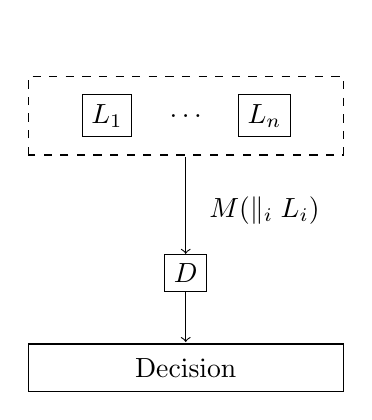
\begin{tikzpicture}
	\node[draw]		(0)	at (1, 3) 		{$L_1$};
  \node[] (fake) [above of=0]              {}; %for space above the picture
	\node[]			(1)	[right of = 0]	{$\ldots$};
	\node[draw]		(2)	[right of = 1]	{$L_n$};
	\draw[dashed] (0, 2.5) rectangle (4, 3.5);
	\node[]			(3) at (2, 2.6) {};
	\node[draw]		(4) at (2, 1) {$D$};
	\draw[->] (3) -- (4);
	\node[]	at (3, 1.8) {$M(\parallel_{i} L_i)$};
	\node[]		(5) [below of = 4] {};
	\draw[->] (4) -- (5);
	\draw[] (0, -.5) rectangle (4, 0.1);
	\node[]			(3) at (2, -.2) {Decision};
\end{tikzpicture}
\caption{Architecture of a system with centralized diagnosis}
\label{fig_centralized}
% \end{figure}
% 
% \begin{figure}[t]
% \centering
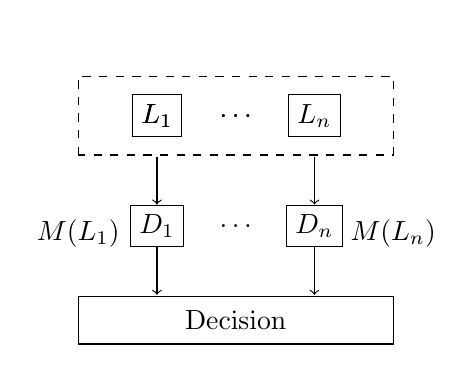
\begin{tikzpicture}
	\node[draw]		(0)	at (1, 3) 		{$L_1$};
   \node[] (fake) [above of=0]              {}; %for space above the picture
	\node[]		(0)	at (1, 3) 		{$L_1$};
	\node[]			(1)	[right of = 0]	{$\ldots$};
	\node[draw]		(2)	[right of = 1]	{$L_n$};
	\draw[dashed] (0, 2.5) rectangle (4, 3.5);

	\node[]			(000)	at (1, 2.6) {};
	\node[draw]		(00) [below of = 000] {$D_1$};
	\node[]			(10) [below of = 00] {$$};
	\draw[->] (000) -- (00);
	\draw[->] (00) -- (10);

	\node[]			(1)	[right of = 0]	{$\ldots$};
	\node[]			(11)[right of = 00]	{$\ldots$};

	\node[]			(222)	at (3, 2.6) {};
	\node[draw]		(22) [below of = 222] {$D_n$};
	\node[]			(20) [below of = 22] {$$};
	\draw[->] (222) -- (22);
	\draw[->] (22) -- (20);

	\node[]	at (0, 1.5) {$M(L_1)$};
	\node[]	at (4, 1.5) {$M(L_n)$};

	\draw[] (0, 0.7) rectangle (4, 0.1);
	\node[]			(3) at (2, .4) {Decision};
\end{tikzpicture}
\caption{Architecture of a system with decentralized diagnosis}
\label{fig_decentralized}
\end{figure}

\begin{figure}[t]
\centering
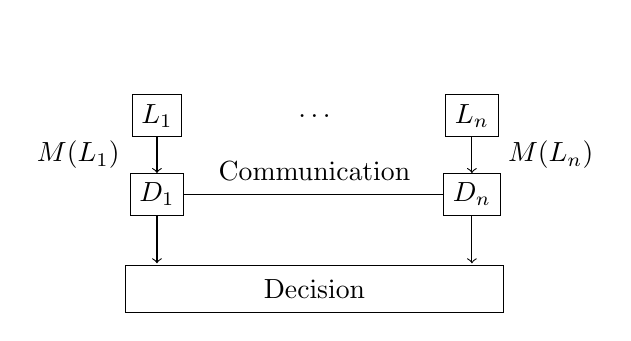
\begin{tikzpicture}
	\node[draw]		(0)	at (1, 2) 		{$L_1$};
  \node[] (fake) [above of=0]              {}; %for space above the picture
	\node[draw]		(00) [below of = 0] {$D_1$};
% 	\node[draw]		(p0) [below of = 00] {Decision$_1$};
	\node[]			(10) [below of = 00] {};
	\draw[->] (0) -- (00);
	\draw[->] (00) -- (10);

	\node[]			(1)	at (3, 2)	{$\ldots$};
	\node[] at (3, 1.3) {Communication};

	\node[draw]		(2)	at (5, 2) 		{$L_n$};
	\node[draw]		(22) [below of = 2] {$D_n$};

	\draw[] (.6, 0.1) rectangle (5.4, -0.5);
	\node[]			(3) at (3, -0.2) {Decision};

% 	\node[draw]		(p2) [below of = 22] {Decision$_n$};
	\node[]			(20) [below of = 22] {};
	\draw[->] (2) -- (22);
	\draw[->] (22) -- (20);
	\draw[] (00) -- (22);

	\node[]	at (0, 1.5) {$M(L_1)$};
	\node[]	at (6, 1.5) {$M(L_n)$};
\end{tikzpicture}
\caption{Architecture of a system with distributed diagnosis}
\label{fig_distributed}
\end{figure}

\subsection{Centralized diagnosability}
This architecture refers to a global model (language).If the system is modular,
then the global language is built by the parallel composition of the local
languages. All the observations are performed at one site. In this architecture
only one diagnoser $D$ \cite{sampath_diagnosability_1995} is constructed. Upon
the current state of the diagnoser a decision on the fault occurrence is made.
The structure is depicted in Figure \ref{fig_centralized}.

\subsection{Decentralized diagnosability}
This approach also exploits the entire model of a system built from its modules,
but several local sites perform observations using only local diagnosers.
The diagnosers do not communicate to each other, but they provide necessary
information (via a protocol) to a central decision node. This architecture is
depicted in Figure \ref{fig_decentralized}.

\subsection{Distributed diagnosability}
The architecture is depicted in Figure \ref{fig_distributed}.
The distributed approach does not require to built the entire model of the
system. The architecture implies that the system has a set of observation spots,
and each spot observes only one module of the system. A communication among
observation spots is possible in order to make a decision about a fault
occurrence.

% In \cite{basilio_computation_2012} the authors search for a
% minimal even-base, e.g. a minimal set of observable events, that ensures
% diagnosability for a given language (module).

The notion of modular diagnosability meets the same architectural implications,
and we refer to it as to the distributed approach when the amount of information
the observation spots communicate to each other is equal to zero. 

For the distributed approach, in general, the bigger the observation spots for
the same system, the less communications among the spots is required.
Figure \ref{fig:curves} shows that the average size of a composed module grows
while the system's modules are composed together (we imply that each module is
represented by automata, and the size of a module is reflected by the number of
states of a corresponding automaton).
The shape of this curve depends mostly on the order the modules are taken for
the composition, but the initial point, when the system has maximal modularity,
and the final point, when all the modules are composed into one monolithic
model, remain the same. Assuming that the system is diagnosable, the average
size of a diagnoser grows much faster, since it is exponential with respect to
the average size of a module, in the worst case.
The amount of events the diagnosers have to exchange among each other, in order
to decide if a fault occurred, is decreasing. The reason the diagnosers require
less event for decision making is due to the fact that they become more
self-sufficient, since amount of observable events available for each
diagnoser without communications is growing. Thus, the events exchange rate
decreases down to the point where no communications is required to make a
decision about the faults occurrence. That is the point when the system becomes
modular diagnosable (the notion of modular diagnosability was introduced in
\cite{contant_diagnosability_2006}). The following composition of the modules
does not affect diagnosability, and leads only to the growth of the modules' and
diagnosers' sizes.

In our approach, given a system with an initial natural modularity, we search
for a point, when the system is modular diagnosable. If the system is diagnosable,
then this point can always be found. The modules corresponding to that
modularity we call \emph{virtual}, since they differ from natural modules and
used only to build diagnosers.

\begin{figure}[t]
\centering
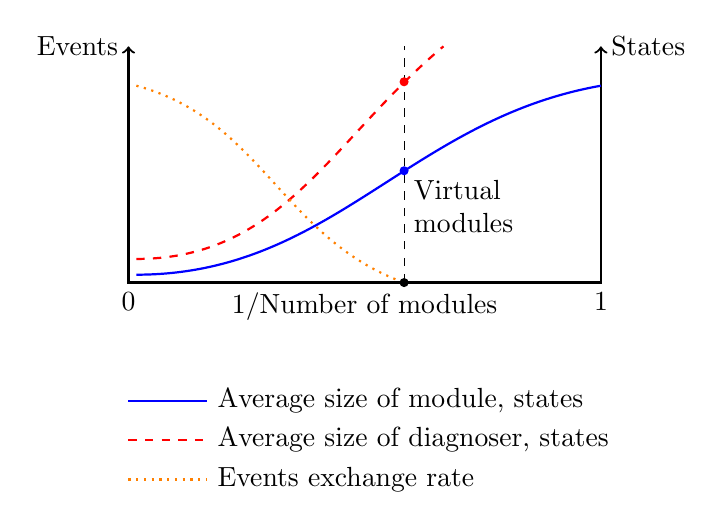
\begin{tikzpicture}
% \draw[help lines] (0,0) grid (5,3);
% Axis 
\draw [thick, <->] 
	(0,3) node[left]{Events} -- 
	(0,0) node[below]{0} -- 
	(6,0) node[below]{1} -- 
	(6,3) node[right]{States};
\node [below] at (3,0) {1/Number of modules};
% Curve of the average size of modules
\draw[blue, thick] (0.1,.1) to [out=0,in=-170] (6,2.5); 
% Curve of the average size of diagnosers
\draw[red, thick, dashed] (0.1,.3) to [out=0,in=-140] (4,3); 
% Curve of the amount of communication
\draw[orange, thick, dotted] (0.1,2.5) to [out=-15,in=160] (3.5,0); 
% Line of the point with virtual modularity
\draw[dashed] (3.5,0) -- (3.5,3);
% Point of virtual modularity  
\draw [fill] (3.5,0) circle [radius=0.05];
\draw [fill, blue] (3.5,1.42) circle[radius=0.05] 
	node[align=left, black, below right] {Virtual\\ modules}; 
\draw [fill, red] (3.5,2.55) circle [radius=0.05];
% Legend
\draw[blue, thick] (0,-1.5) -- (1,-1.5)
	node[black, right] {Average size of module, states};
\draw[red, thick, dashed] (0,-2) -- (1,-2)
	node[black, right] {Average size of diagnoser, states};
\draw[orange, thick, dotted] (0,-2.5) -- (1,-2.5) 
	node[black, right] {Events exchange rate};

\end{tikzpicture}
\caption{Size of modules, diagnosers, and events exchange rate, changing 
with respect to the degree of modularity of the system}
\label{fig:curves}
\end{figure}



\subsection{Diagnosability of a Modular System}

Diagnosability analysis uses a notion of a faulty language to describe the
faulty behaviour of a discrete-event system. This section discuses design issues
related to representations of the faulty language and focuses on a definition
of modular diagnosability.

The faulty behavior is usually modeled by introducing fault events or by faulty
specifications. We refer to this approaches as to \emph{event-based} and
\emph{specification-based} correspondingly. All the aforementioned works exploit
the event-based approach, whereas the works \cite{zhou_decentralized_2008} and
\cite{sartini_methodology_2010} are examples of the specification-based one.

In the event-based approach fault events are a special type of event such that
$\Sigma_{uo}$ can be disjointed into the sets of faults $\Sigma_f$ and
non-faults $\Sigma_{uo}\backslash \Sigma_f$. A string containing a fault event
is called \emph{faulty string}. A set of faulty strings is called \emph{faulty
language}, i.e. formally 
$$L_f := \{ s \in L \mid \sigma \in s, \sigma \in \Sigma_f\}.$$ 
By definition, the faulty language is not necessarily prefix-closed,
$L_f \subseteq \overline{L_f}$. Thus, in the event-based approach the language
of the system can be partitioned into faulty and non-faulty languages, where the
\emph{non-faulty language} is defined as $L_{nf} := L \backslash L_f$.

In the case of the specification-based approach the faulty specification allows
us to define undesired behavior when the fault events are not necessarily
introduced. In this case this behaviour can be represented by a marked
language $L_f := L_m \subseteq L$. Labeling automata's states for the same
purpose can be considered as an equal technique.

Different types of undesired behaviours (or types of faults) are defined by
partitioning $\Sigma_f$ into subsets (not necessarily disjoint) or by several
faulty specifications for the same language. 

A faulty language defined in the event-based approach can be simply converted
into a faulty specification by marking faulty strings, and erasing fault events.
Then, we can assume that if fault events are defined, then faulty specifications
can also be defined. Consequently, a set of different types of faults requires a
corresponding set of specifications.
Thus, a method suitable for the specification-based approach implies that it can
be adopted for the event-based approach. In this paper, for the sake of
unification, we use specification-based approach. For this reason the
definitions of diagnosability originally developed by their authors for the
event-based approach are slightly modified with no loss of meaning.

For the sake of simplicity, in the following we assume that there is only one
type of fault, and that the language of the system is live.

We define \emph{diagnosability of a fault} as follows:
\begin{definition} 
\label{def:fault_is_diag}
Given a system's language $L$ with a fault defined by the sublanguage $L_f$. The
fault is diagnosable if there is no two strings in the language $L$ with the
same observation such that one string is faulty and of arbitrary cardinality,
and another is non-faulty, i.e. if the following holds:
\end{definition}
\begin{equation}
\begin{array}{l}
	\forall(s \in L_f, t \in L_f/s) 
	\\
	(\exists n \in \mathbb{N})
	(|t| \geq n) 
	\\
	\left[ M(st) \cap M(L_{nf}) = \emptyset \right].
\end{array}
\end{equation}

We define \emph{diagnosability property of a language} as follows:
\begin{definition}
The language is diagnosable if all its faults are diagnosable.
\end{definition}
The two above definitions altogether are similar to the Definition 1 in
\cite{sampath_diagnosability_1995}. We recall the statement in
\cite{contant_diagnosability_2006} proved by Theorem 2, that the global
language of the system is not diagnosable only if it exists at least one
non-diagnosable local language. If all the local languages are diagnosable then the global
language is diagnosable. We refer to this property as to a local diagnosability
property:

\begin{definition}[Local diagnosability] Given the set of languages
$\{L_{i \in I}\}$. The global language $L := \parallel L_i$ is
diagnosable locally if each local language $L_i$ is diagnosable, i.e. if
the following holds:
\end{definition}
\begin{equation}
\begin{array}{l}
	\forall(i \in I, s \in L_{i,f}, t \in L_{i,f}/s)
	\\
	(\exists n \in \mathbb{N})
	(|t| \geq n)
	\\
	\left[ M_i(st) \cap M_i(L_{i,nf}) = \emptyset \right].
\end{array}
\end{equation}

The definition of modular diagnosability extends the definition of local
diagnosability as it takes into account the case when a faulty string locally
indistinguishable in one module becomes distinguishable due to the
composition with another module:

\begin{definition}[Modular diagnosability] Given the set of local languages
$\{L_{i \in I}\}$ and its corresponding sets $\{L_{i,f}\}$ and
$\{L_{i,nf}\}$. The global language $L := \parallel L_i$ is \emph{modularly
diagnosable} with respect to
$M_i: \Sigma^* \rightarrow \Sigma_{i,o}^*$ 
if the following holds:
\end{definition}
\begin{equation}
\begin{array}{l}
	\forall(i \in I, s \in L_{i,f}, t \in L_{i,f}/s)
	\\
	(\exists n \in \mathbb{N})
	(|t| \geq n)
	\\
	\left[ M_i(P_i^{-1}(st)) \cap M_i(P_i^{-1}(L_{i,nf})) = \emptyset \right].
\end{array}
\end{equation}

It was proved in \cite{contant_diagnosability_2006} by Theorem 2, Part 2 
that the local diagnosability implies the modular diagnosability\footnote{In
\cite{zhou_decentralized_2008} the authors show that the local diagnosability
and modular diagnosability are not comparable but they have a different setup
for the problem.}, i.e.
\begin{equation}
\begin{array}{l}
	\forall(i \in I, s \in L_{i,f}, t \in L_{i,f}/s)
	\\
	(\exists n \in \mathbb{N})
	(|t| \geq n)
	\\
	\left[
	\left( M_i(st) \cap M_i(L_{i,nf}) = \emptyset \right)
	\Rightarrow \right.
	\\ 
	\left.
	\left( M_i(P_i^{-1}(st)) \cap M_i(P_i^{-1}(L_{i,nf})) = \emptyset \right)
	\right].
\end{array}
\end{equation}


Recall the Definition \ref{def:fault_is_diag} of the diagnosable fault. If a
module is not diagnosable locally then exist at least two strings in its
language, one is faulty and the other one is not, with the same observation of
arbitrary length, i.e. the strings are \emph{not distinguishable}. The
indistinguishability can disappear if and only if:
$a)$ at least one string is not in its language due to concurrency with other
module, and then the strings would be distinguishable locally - the verification
of the modular diagnosability property is devoted to find if this is the case;
$b)$ indistinguishability is broken globally by interleaving sequences of the
module's events with observable events of other modules. The later case is
expressed in the following conjecture:
\begin{conjecture} Given a system of two modules with languages $L_1$ and $L_2$,
and the global language $L := L_1 \parallel L_2$. Suppose there is only
one faulty string $s \in L_1$ such that it is not distinguishable from at least one
string of $L_1\backslash s$. Thus, $L_1$ is not locally diagnosable. Suppose the
system is not modular diagnosable. Then the global language $L$ is diagnosable
only if all the strings $t \in P_1^{-1}(s)$ change their observation due to 
the composition with the language $L_2$.
\end{conjecture}

The above conjecture gives the insight into the underlining idea of our
approach. If we find a module which makes the faulty string distinguishable
then the composition of that module with a faulty one would result in a new
module satisfying the property of local diagnosability, thus improving
the modular diagnosability property of the system. In the following section we
provide a formal description of the problem.


